\section{Einführung}
Resonanzkreise werden im allgemeinen als Frequenzfilter genutzt, um das Empfangen von nur speziellen Frequenzen zu ermöglichen.
\subsection{Serienresonanzkreis}
Der Strom $I$ wird wie folgt berechnet:
\begin{equation}
  |I|=\frac{|U|}{\sqrt{R^2+(\omega L-\frac{1}{\omega C})^2}}
  \label{eq:serienstrom}
\end{equation}
\subsection{Parallelresonanzkreis}
\section{Versuch: Serienresonanzkreis}
Wir überprüfen den aus \cref{eq:serienstrom} erwarteten Zusammenhang, indem wir die obigen Daten mit gnuplot gegen die Funktion $I(C)$ plotten. Wir erhalten:
\begin{table}[H]
  \centering
  \begin{tabular}{c c c c} \toprule
    Parameter & für \SI{500}{\ohm} & für \SI{200}{\ohm} & für \SI{0}{\ohm} \\ \midrule
    $R$ & \SI{694(326)}{\ohm} & \SI{385(283)}{\ohm}  & \SI{30(2041)}{\ohm} \\
    $L$ & \SI{94.06(53)}{\henry} & \SI{93.88(24)}{\henry} & \SI{93.84(16)}{\henry} \\ \bottomrule 
  \end{tabular}
  \caption{Fit}
  \label{tab:serienfit}
\end{table}

\begin{figure}[H]
\centering
\begin{tikzpicture}
  \begin{axis}[
    width=15 cm,
    height=9 cm,
    xmin=75, xmax=105,
    ymin=0, ymax=6,
    xlabel={$1/C$ [\si{mF^{-1}}]},
    ylabel={$I$ [\si{mA}]},
    domain=50:250,
    cycle list name=color list
  ]
  \addplot+ plot [only marks,mark=x]  table[x expr=1/\thisrowno{0}, y index=2] {serie.csv};
  \addplot+ plot [only marks,mark=asterisk]  table[x expr=1/\thisrowno{3}, y index=5] {serie.csv};
  \addplot+ plot [only marks,mark=square]  table[x expr=1/\thisrowno{6}, y index=8] {serie.csv};
  \pgfplotsset{cycle list shift=-3};
  \addplot+ plot [samples=500, mark=none] {1000*2.01/sqrt(694^2+(1000*94.06-x/(1000*10^(-6)))^2)};
  \addplot+ plot [samples=500, mark=none] {1000*2.01/sqrt(385^2+(1000*93.88-x/(1000*10^(-6)))^2)};
  \addplot+ plot [samples=500, mark=none] {1000*2.01/sqrt(30^2+(1000*93.84-x/(1000*10^(-6)))^2)};
  \end{axis}
\end{tikzpicture}
\caption{Fit der dynamischen Viskosität von Luft}
\label{fig:dynviskos}
\end{figure}
\section{Versuch: Parallelresonanzkreis}
An dem Aufbau \ref{fig:aufbauparallel} wird eine Spannung von $U_\approx=\pm 5V$ mit einer Frequenz von $F=(1 \pm 0,005) kHz$ angelegt und es wird der Spannungsabfall am $10\Omega$ Widerstand für unterschiedliche Kapazitäten und Widerstände $R_p$ bestimmt. Der Fehler der Kapazität war mit $1\% $ der eingestellten Kapazität gegeben und der Fehler der Spannung ergab sich aus der Genauigkeit des Messgeräts.
\begin{figure}[h]
  \centering
  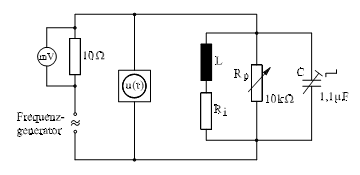
\includegraphics[width=.9\textwidth]{Bauplanparall.png}
  \caption{Aufbau eines Parallelresonanzkreises}
  \label{fig:aufbauparallel}
\end{figure}
 Die Stromstärke konnte nun nach der Formel $I=\frac{U}{R}$ berechnet werden. Mit der gleichen Formel wurde mit Hilfe der Gauß'sches Fehlerfortpflanzung der Fehler der Stromstärke bestimmt (Siehe Anhang).
\subsection{$10 k\Omega$ Widerstand}
\begin{table}[h]
  \centering
  
    \begin{tabular}{rrrrrr}
    \toprule
    Kapazität C [µF] & Fehler [µF] & Spannung U [mV] & Fehler [mV] & Stromstärke I [mA] & Fehler [mA] \\
    \midrule
    
        0,000 & 0,000 & 62,900 & 0,100 & 6,290 & 0,315 \\
        0,050 & 0,001 & 52,100 & 0,100 & 5,210 & 0,261 \\
        0,100 & 0,001 & 41,500 & 0,100 & 4,150 & 0,208 \\
        0,147 & 0,001 & 31,500 & 0,100 & 3,150 & 0,158 \\
        0,150 & 0,002 & 30,800 & 0,100 & 3,080 & 0,154 \\
        0,180 & 0,002 & 24,500 & 0,100 & 2,450 & 0,123 \\
        0,210 & 0,002 & 18,300 & 0,100 & 1,830 & 0,092 \\
        0,240 & 0,002 & 12,600 & 0,100 & 1,260 & 0,064 \\
        0,253 & 0,003 & 10,500 & 0,100 & 1,050 & 0,053 \\
        0,270 & 0,003 & 8,400 & 0,100 & 0,840 & 0,043 \\
        0,289 & 0,003 & 7,400 & 0,100 & 0,740 & 0,038 \\
        0,300 & 0,003 & 7,900 & 0,100 & 0,790 & 0,041 \\
        0,321 & 0,003 & 10,500 & 0,100 & 1,050 & 0,053 \\
        0,330 & 0,003 & 12,000 & 0,100 & 1,200 & 0,061 \\
        0,360 & 0,004 & 17,800 & 0,100 & 1,780 & 0,090 \\
        0,390 & 0,004 & 24,000 & 0,100 & 2,400 & 0,120 \\
        0,420 & 0,004 & 30,500 & 0,100 & 3,050 & 0,153 \\
        0,425 & 0,004 & 31,500 & 0,100 & 3,150 & 0,158 \\
        0,450 & 0,005 & 37,000 & 0,100 & 3,700 & 0,185 \\
        0,500 & 0,005 & 47,600 & 0,100 & 4,760 & 0,238 \\
        0,900 & 0,009 & 132,200 & 0,100 & 13,220 & 0,661 \\
    
    \bottomrule
    \end{tabular}
  \caption{Messwerte mit einem $10 k\Omega$ Widerstand}
  \label{tab:10kparallel}
\end{table}

Im folgenden wurde die Werte von C und I im Diagramm aufgetragen.
\begin{figure}[h]
  \centering
  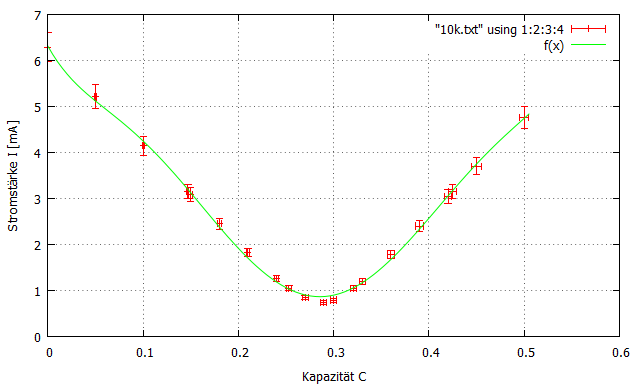
\includegraphics[width=.9\textwidth]{10k.png}
  \caption{$10k\Omega$ Widerstand}
  \label{fig:10k}
\end{figure}

Dem anscheinend polynomischen Verlaufs nach wurden die Messwerte beider Prozesse zusammen gegen die Funktion $I(C)=a\cdot x^6+b\cdot x^5+c\cdot x^4+d\cdot x^3+e\cdot x^2+f\cdot x+g$ mit \emph{gnuplot} nach dem \emph{least-squares}-Verfahren gefittet.
\begin{table}[H]
  \centering
  \begin{tabular}{c | c | c }
    Variabel & Wert & Fehler\\ \hline
    a  & 14329,9 & $\pm 4004$\\
    b & -24283,7 & $\pm6033$\\
    c  & 14789,3 & $\pm 3449$\\
    d  & -3881,36 & $\pm 930$\\
    e  & 429,052 & $\pm 118,6$\\
    f  & -37,299 & $\pm 6,064$\\
    g  & 6,311 & $\pm 0,088$\\
  \end{tabular}
  \caption{Linearer Fit zu Abbildung \ref{fig:10k}}
  \label{tab:fit10k}
\end{table}

Daraus ergibt sich ein Minimum von
\begin{equation}
I_{min}=(0,702\pm 0,035)mA \Rightarrow I_{min}\cdot \sqrt{2}=(0,993\pm0,053)mA
\end{equation}
mit $C_{min}=0,285 \mu F$ und $C_{1}=0,257 \mu F$ und $C_{2}=0,314 \mu F$ mit jeweils $1\%$ Fehler.

Für die Spule lässt sich nun sagen, dass
\begin{equation}
L=\frac{1}{(2\pi f)^2\cdot C}=88,88mH
\end{equation}
\begin{equation}
\Delta L =\sqrt{(\frac{\Delta f}{2\pi^2 f^3 C})^2+(\frac{\Delta C}{2\pi^2 f^2 C^2})^2}=1,24mH
\end{equation}
So ergibt sich für die Spule $L=(88,88 \pm 1,24)mH$.

Der Verlustwiderstand der Schaltung ergibt sich aus
\begin{equation}
R_1= \frac{1}{2\pi f (C_2-C_1)}=2792,192\Omega
\end{equation}
\begin{equation}
\Delta R_1 = \sqrt{ \left( \dfrac{\Delta f}{\pi f^2 (C_2 - C_1)} \right)^2 + \left( \dfrac{\Delta C_2}{\pi f (C_2 - C_1)} \right)^2 + \left( \dfrac{\Delta C_1}{\pi f (C_2 - C_1)} \right)^2}=27,82\Omega
\end{equation}

\newpage
\subsection{$\infty$ Widerstand}

\begin{table}[h]
  \centering
  
    \begin{tabular}{rrrrrr}
    \toprule
    Kapazität C [µF] & Fehler [µF] & Spannung U [mV] & Fehler [mV] & Stromstärke I [mA] & Fehler [mA] \\
    \midrule
    0,000 & 0,000 & 63,000 & 0,100 & 6,300 & 0,330 \\
        0,080 & 0,001 & 45,600 & 0,100 & 4,560 & 0,249 \\
        0,110 & 0,001 & 39,200 & 0,100 & 3,920 & 0,220 \\
        0,140 & 0,001 & 32,600 & 0,100 & 3,260 & 0,191 \\
        0,170 & 0,002 & 26,000 & 0,100 & 2,600 & 0,164 \\
        0,200 & 0,002 & 19,500 & 0,100 & 1,950 & 0,140 \\
        0,230 & 0,002 & 13,100 & 0,100 & 1,310 & 0,120 \\
        0,260 & 0,003 & 7,100 & 0,100 & 0,710 & 0,106 \\
        0,269 & 0,003 & 5,600 & 0,100 & 0,560 & 0,104 \\
        0,289 & 0,003 & 4,000 & 0,100 & 0,400 & 0,102 \\
        0,305 & 0,003 & 5,600 & 0,100 & 0,560 & 0,104 \\
        0,320 & 0,003 & 8,300 & 0,100 & 0,830 & 0,108 \\
        0,350 & 0,004 & 14,600 & 0,100 & 1,460 & 0,124 \\
        0,380 & 0,004 & 21,100 & 0,100 & 2,110 & 0,145 \\
        0,410 & 0,004 & 27,900 & 0,100 & 2,790 & 0,172 \\
        0,440 & 0,004 & 34,400 & 0,100 & 3,440 & 0,199 \\
        0,470 & 0,005 & 41,000 & 0,100 & 4,100 & 0,228 \\
        0,500 & 0,005 & 47,400 & 0,100 & 4,740 & 0,257 \\
        \bottomrule
    
    \end{tabular}
  \label{tab:addlabel}
  \caption{Messwerte mit einem unendlichem Widerstand}
\end{table}

Im folgenden wurde die Werte von C und I im Diagramm aufgetragen.
\begin{figure}[h]
  \centering
  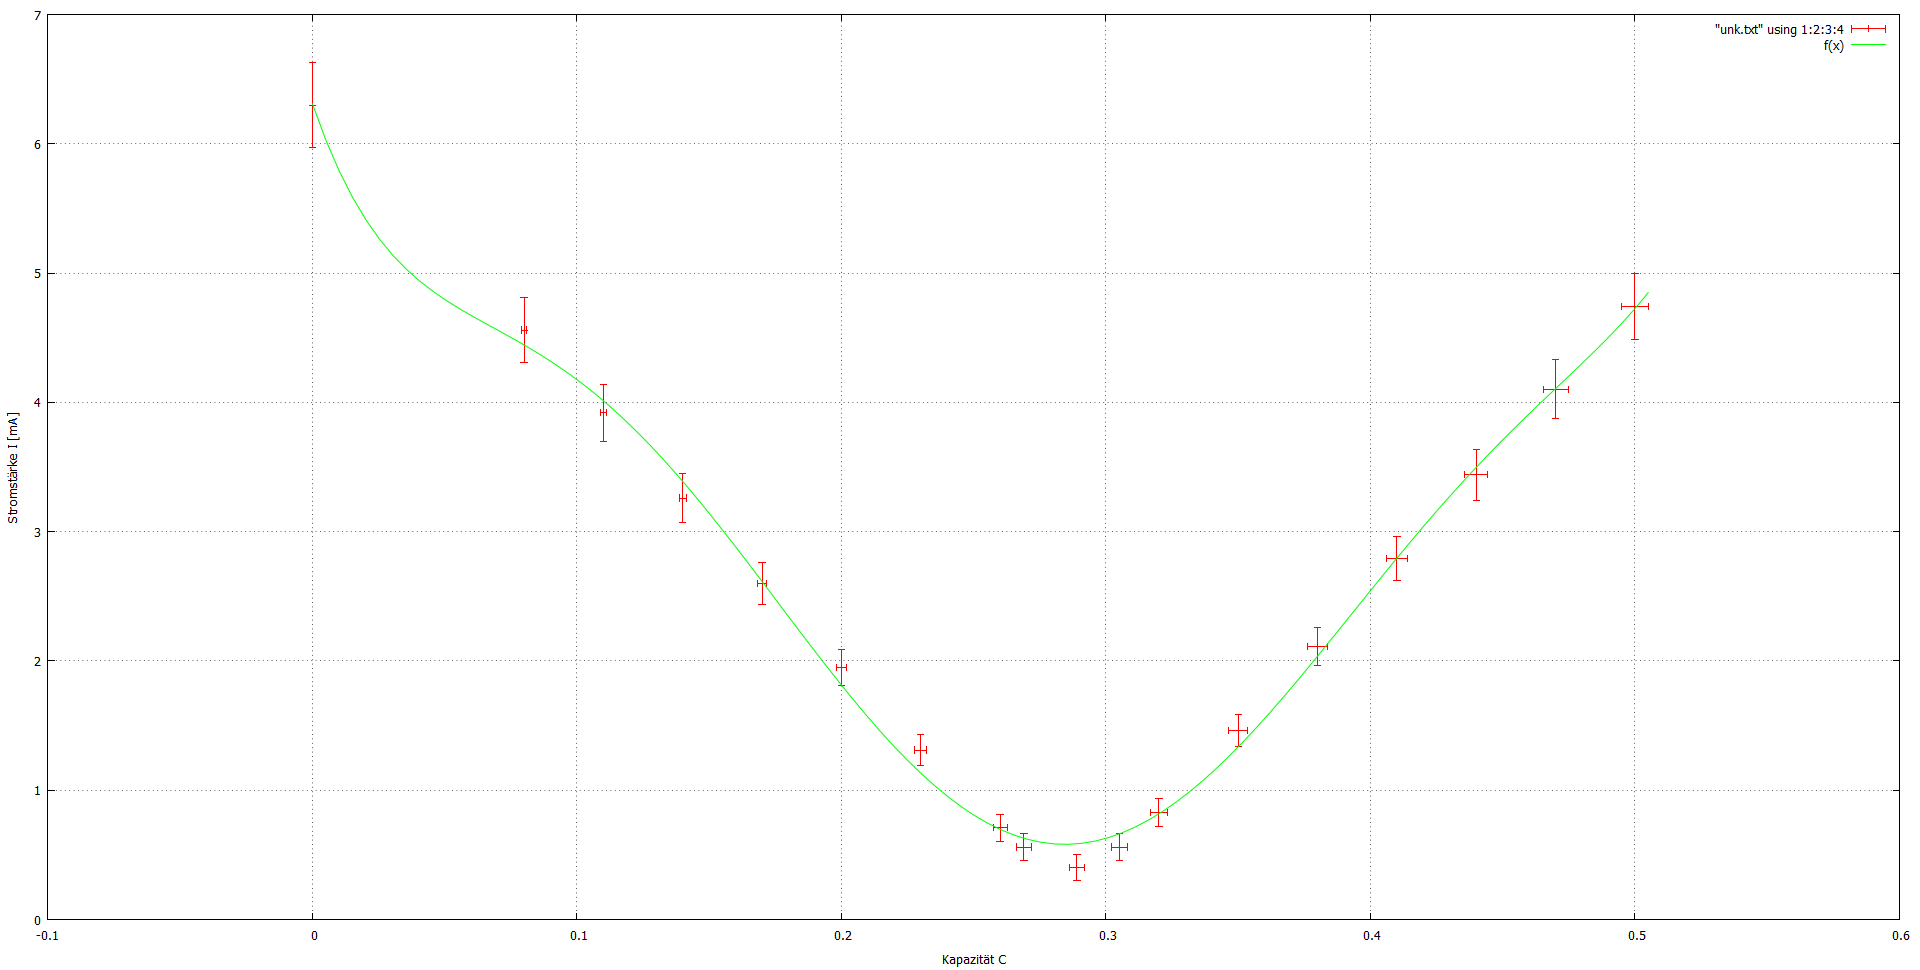
\includegraphics[width=.9\textwidth]{unendlich.png}
  \caption{$\infty\Omega$ Widerstand}
  \label{fig:unendlich}
\end{figure}

Dem anscheinend polynomischen Verlaufs nach wurden die Messwerte beider Prozesse zusammen gegen die Funktion $I(C)=a\cdot x^6+b\cdot x^5+c\cdot x^4+d\cdot x^3+e\cdot x^2+f\cdot x+g$ mit \emph{gnuplot} nach dem \emph{least-squares}-Verfahren gefittet.
\begin{table}[H]
  \centering
  \begin{tabular}{c | c | c }
    Variabel & Wert & Fehler\\ \hline
    a  & 27020,7 & $\pm 6518$\\
    b & -44927,8 & $\pm10090$\\
    c  & 27579,5 & $\pm 5963$\\
    d  & -7512,98 & $\pm 1669$\\
    e  & 901,99 & $\pm 219,9$\\
    f  & -59,7594 & $\pm 11,03$\\
    g  & 6,309 & $\pm 0,122$\\
  \end{tabular}
  \caption{Linearer Fit zu Abbildung \ref{fig:unendlich}}
  \label{tab:fitinfi}
\end{table}

Daraus ergibt sich ein Minimum von
\begin{equation}
I_{min}=(0,580\pm 0,037)mA \Rightarrow I_{min}\cdot \sqrt{2}=(0,820\pm0,047)mA
\end{equation}
mit $C_{min}=0,285 \mu F$ und $C_{1}=0,25 \mu F$ und $C_{2}=0,32 \mu F$ mit jeweils $1\%$ Fehler.

Für die Spule lässt sich nun sagen, dass
\begin{equation}
L=\frac{1}{(2\pi f)^2\cdot C}=88,88mH
\end{equation}
\begin{equation}
\Delta L =\sqrt{(\frac{\Delta f}{2\pi^2 f^3 C})^2+(\frac{\Delta C}{2\pi^2 f^2 C^2})^2}=1,24mH
\end{equation}
So ergibt sich für die Spule $L=(88,88 \pm 1,24)mH$.

Der Verlustwiderstand der Schaltung ergibt sich aus
\begin{equation}
R_1= \frac{1}{2\pi f (C_2-C_1)}=2273,642\Omega
\end{equation}
\begin{equation}
\Delta R_1 = \sqrt{ \left( \dfrac{\Delta f}{\pi f^2 (C_2 - C_1)} \right)^2 + \left( \dfrac{\Delta C_2}{\pi f (C_2 - C_1)} \right)^2 + \left( \dfrac{\Delta C_1}{\pi f (C_2 - C_1)} \right)^2}=29,00\Omega
\end{equation}

\subsection{$2k\Omega$ Widerstand}
\begin{table}[]
  \centering
 
    \begin{tabular}{rrrrrr}
    \toprule
    Kapazität C [µF] & Fehler [µF] & Spannung U [mV] & Fehler [mV] & Stromstärke I [mA] & Fehler [mA] \\
    \midrule
    0,000 & 0,000 & 64,200 & 0,100 & 6,420 & 0,336 \\
    0,080 & 0,001 & 48,200 & 0,100 & 4,820 & 0,261 \\
    0,110 & 0,001 & 42,500 & 0,100 & 4,250 & 0,235 \\
    0,140 & 0,001 & 37,000 & 0,100 & 3,700 & 0,210 \\
    0,170 & 0,002 & 31,600 & 0,100 & 3,160 & 0,187 \\
    0,198 & 0,002 & 27,100 & 0,100 & 2,710 & 0,168 \\
    0,200 & 0,002 & 26,800 & 0,100 & 2,680 & 0,167 \\
    0,230 & 0,002 & 22,800 & 0,100 & 2,280 & 0,152 \\
    0,260 & 0,003 & 20,300 & 0,100 & 2,030 & 0,142 \\
    0,289 & 0,003 & 19,200 & 0,100 & 1,920 & 0,139 \\
    0,320 & 0,003 & 20,500 & 0,100 & 2,050 & 0,143 \\
    0,350 & 0,004 & 23,600 & 0,100 & 2,360 & 0,155 \\
    0,375 & 0,004 & 27,100 & 0,100 & 2,710 & 0,168 \\
    0,380 & 0,004 & 27,800 & 0,100 & 2,780 & 0,171 \\
    0,410 & 0,004 & 33,000 & 0,100 & 3,300 & 0,193 \\
    0,440 & 0,004 & 38,400 & 0,100 & 3,840 & 0,216 \\
    0,470 & 0,005 & 44,200 & 0,100 & 4,420 & 0,243 \\
    0,500 & 0,005 & 49,800 & 0,100 & 4,980 & 0,268 \\
    \bottomrule
    \end{tabular}
  \label{tab:addlabel}
   \caption{Messwerte mit einem $2 k\Omega$ Widerstand}
\end{table}
Im folgenden wurde die Werte von C und I im Diagramm aufgetragen.
\begin{figure}[]
  \centering
  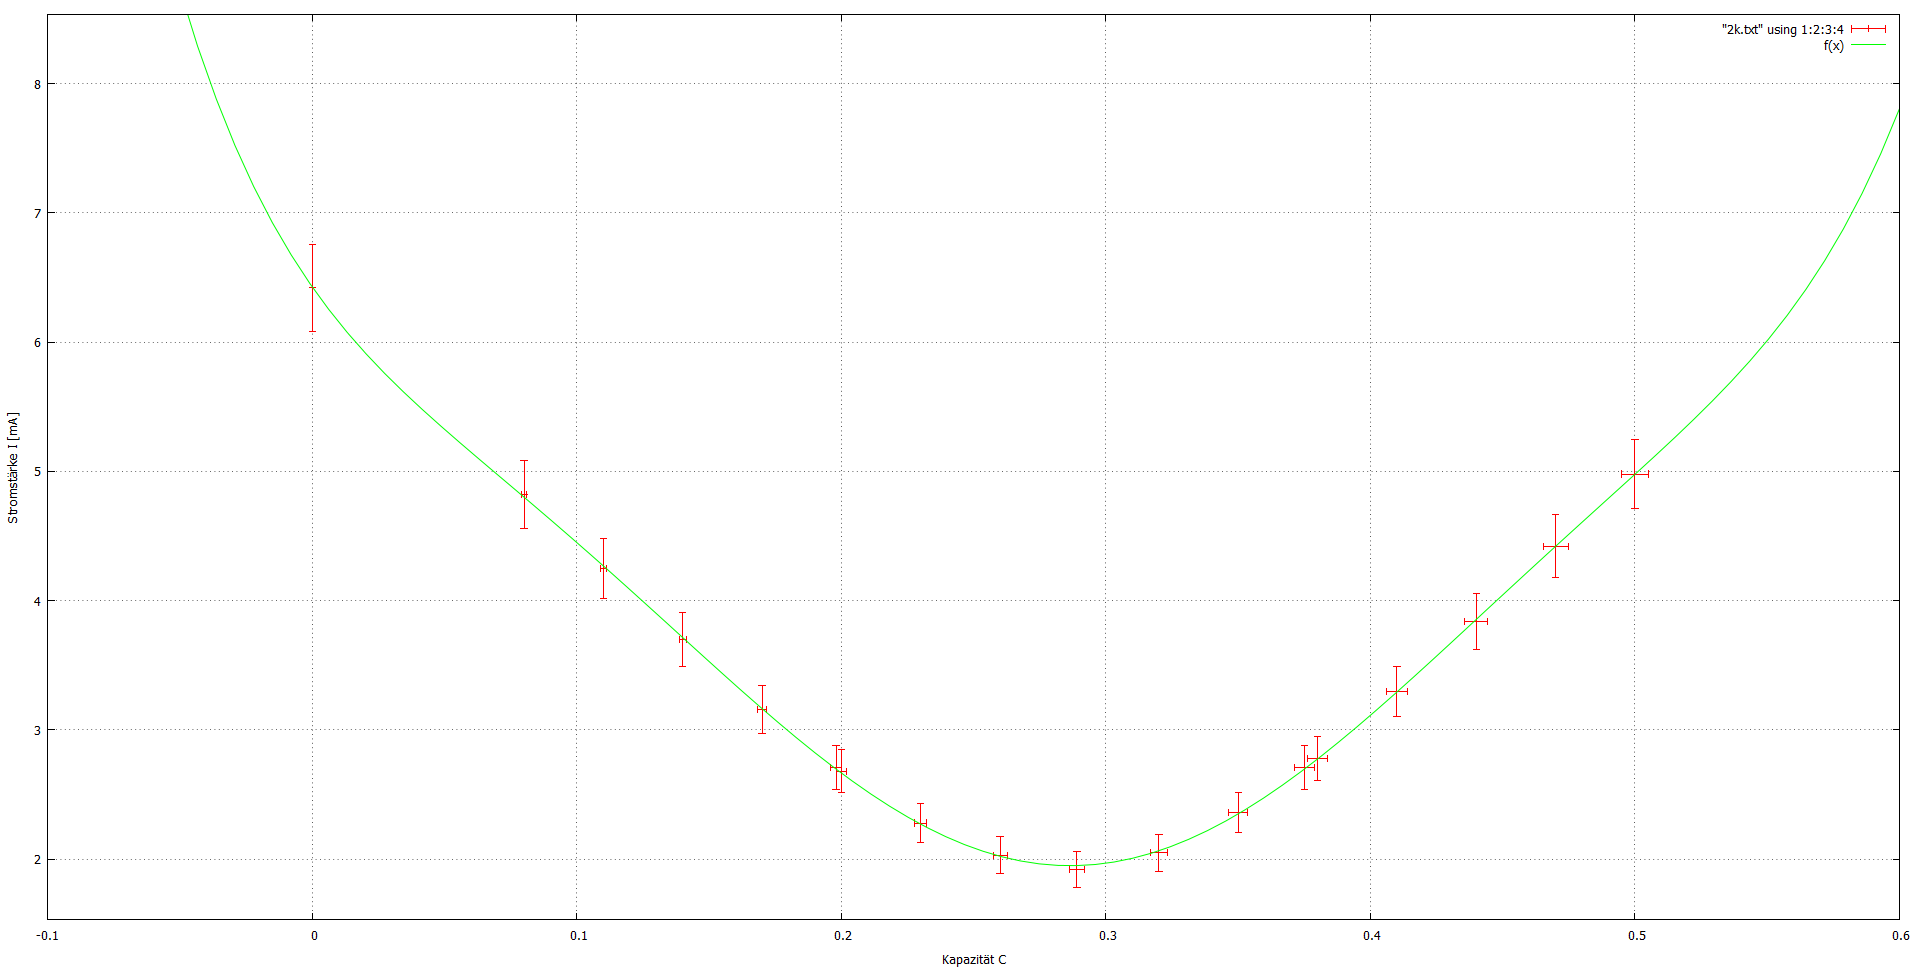
\includegraphics[width=.9\textwidth]{2k.png}
  \caption{$2k\Omega$ Widerstand}
  \label{fig:2k}
\end{figure}

Dem anscheinend polynomischen Verlaufs nach wurden die Messwerte beider Prozesse zusammen gegen die Funktion $I(C)=a\cdot x^6+b\cdot x^5+c\cdot x^4+d\cdot x^3+e\cdot x^2+f\cdot x+g$ mit \emph{gnuplot} nach dem \emph{least-squares}-Verfahren gefittet.
\begin{table}[H]
  \centering
  \begin{tabular}{c | c | c }
    Variabel & Wert & Fehler\\ \hline
    a  & 6919,65 & $\pm 909,9$\\
    b & -11829,1 & $\pm1414$\\
    c  & 7273,85 & $\pm 838,5$\\
    d  & -1880,89 & $\pm235,2$\\
    e  & 220,707& $\pm 30,92$\\
    f  & -29,17 & $\pm 1,547$\\
    g  & 6,42 & $\pm 0,017$\\
  \end{tabular}
  \caption{Linearer Fit zu Abbildung \ref{fig:2k}}
  \label{tab:fit2k}
\end{table}

Daraus ergibt sich ein Minimum von
\begin{equation}
I_{min}=(1,95\pm 0,140)mA \Rightarrow I_{min}\cdot \sqrt{2}=(2,7577\pm0,160)mA
\end{equation}
mit $C_{min}=0,285 \mu F$ und $C_{1}=0,194 \mu F$ und $C_{2}=0,38 \mu F$ mit jeweils $1\%$ Fehler.

Für die Spule lässt sich nun sagen, dass
\begin{equation}
L=\frac{1}{(2\pi f)^2\cdot C}=88,88mH
\end{equation}
\begin{equation}
\Delta L =\sqrt{(\frac{\Delta f}{2\pi^2 f^3 C})^2+(\frac{\Delta C}{2\pi^2 f^2 C^2})^2}=1,24mH
\end{equation}
So ergibt sich für die Spule $L=(88,88 \pm 1,24)mH$.

Der Verlustwiderstand der Schaltung ergibt sich aus
\begin{equation}
R_1= \frac{1}{2\pi f (C_2-C_1)}=855,67\Omega
\end{equation}
\begin{equation}
\Delta R_1 = \sqrt{ \left( \dfrac{\Delta f}{\pi f^2 (C_2 - C_1)} \right)^2 + \left( \dfrac{\Delta C_2}{\pi f (C_2 - C_1)} \right)^2 + \left( \dfrac{\Delta C_1}{\pi f (C_2 - C_1)} \right)^2}=8,56\Omega
\end{equation}

\subsection{Innenwiderstand der Spule}

Bei der direkten Bestimmung des Innenwiderstands der Spule mit Hilfe des Multimeters ergab sich
\begin{equation}
R_{innen}=(18,9\pm0,1)\Omega
\end{equation}

Bei der Bestimmung aus den Resonanzkurven nutzt man den Umstand, dass bei $R_p = \infty$ gilt

\begin{equation}
R_i=\frac{(2\pi f)^2L^2}{R}=31,186
\end{equation}
\section{Diskussion}
\subsection{Parallelresonanzkreis}
Die Werte für die Induktivität der Spule stimmten bei allen Messungen überein, es gab nur Unterschiede außerhalb des Messgenauigkeit. Die Werte für den Innenwiderstand der Spule hingegen weichen deutlich von einander ab. Dies liegt nicht mehr im Rahmen der Messungenauigkeiten und ist auf eine Erwärmung der Spule oder andere Einflüsse zurück zuführen. 
